\chapter{Issue --- タスクとバグを管理する}

\section{この章で学ぶこと}

この章では、GitHubの\textbf{Issue（イシュー）}機能について、その基本的な考え方から実践的な活用方法までを体系的に学びます。具体的には、以下の内容を扱います。

\begin{itemize}
  \item Issueとは何か――プロジェクト管理における「チケット」としての役割
  \item Issue番号の仕組みと、それがリポジトリ全体でどのように管理されるか
  \item Web UIとCLI（GitHub CLI）の両方を使ったIssueの作成方法
  \item バグ報告や機能要望を的確に伝えるための「良いIssueの書き方」
  \item ラベルやマイルストーンを活用した整理・分類の手法
  \item IssueとPull Requestを連携させて、作業の流れを自動化する方法
  \item テンプレートを用いて、チーム全体のIssue品質を底上げする方法
\end{itemize}

ソフトウェア開発では、コードを書くことと同じくらい「何をすべきか」「何が問題か」を正確に記録・共有することが重要です。Issueはまさにその「記録と共有」を担う中核的な機能です。

\section{Issueとは何か}

\subsection{チケットシステムとしてのIssue}

ソフトウェア開発の現場では、日々さまざまな「やるべきこと」が発生します。ユーザーから「この画面が正しく表示されない」というバグ報告が届くこともあれば、チームメンバーから「ダークモードに対応したい」という機能提案が出ることもあります。こうした情報をメールやチャットだけでやり取りしていると、どの問題が未解決で、誰が担当していて、いつまでに対応すべきなのかが分からなくなってしまいます。

この課題を解決するのが\textbf{チケットシステム}（Issue Tracking System）です。Jira、Redmine、Backlogといったツールを聞いたことがある方もいるでしょう。GitHubのIssueは、こうしたチケットシステムの機能をGitHubの中に統合したものです。コードリポジトリと同じ場所でタスクやバグを管理できるため、「コードの変更」と「その変更が何のために行われたか」を自然に紐づけることができます。

Issueは大きく分けて以下の用途で使われます。

\begin{itemize}
  \item \textbf{バグ報告} --- 「この機能が正しく動かない」という問題の記録
  \item \textbf{機能要望} --- 「こんな機能がほしい」という提案
  \item \textbf{タスク管理} --- 「次のリリースまでにやること」のリスト化
  \item \textbf{議論・相談} --- 「この設計方針でよいか」というチーム内の検討
\end{itemize}

\subsection{Issue番号の仕組み}

GitHubでは、IssueとPull Requestが\textbf{同じ番号空間}を共有しています。つまり、最初に作成したIssueが \cmd{\#1}、次に作成したPull Requestが \cmd{\#2}、その次のIssueが \cmd{\#3} というように、リポジトリ内で通し番号が振られます。

この番号はリポジトリごとに独立しており、一度割り当てられた番号は削除しても再利用されません。これは重要な設計上の判断です。なぜなら、コミットメッセージやドキュメントの中で \cmd{\#42} と書けば、それが常に同じIssue（またはPR）を指すことが保証されるからです。もし番号が再利用されてしまうと、過去の参照が別のIssueを指してしまい、混乱の原因になります。

たとえば、コミットメッセージに \cmd{Fix login bug (\#42)} と書いておけば、GitHub上でこの \cmd{\#42} は自動的にリンクになり、クリックすると該当のIssueに飛ぶことができます。この仕組みのおかげで、コードの変更履歴とIssueが自然につながるのです。

\section{Issueの作成}

\subsection{Web UIでの作成}

最も直感的なのは、GitHubのWebインターフェースからIssueを作成する方法です。手順は以下のとおりです。

\begin{enumerate}
  \item リポジトリのページを開き、上部にある「\textbf{Issues}」タブをクリックします
  \item 右上の「\textbf{New issue}」ボタンをクリックします
  \item \textbf{タイトル}を入力します。タイトルは問題の要約を簡潔に書きます（例：「ログインページで404エラーが発生する」）
  \item \textbf{本文}（Description）にMarkdown形式で詳細を記述します
  \item 右側のサイドバーから、必要に応じて\textbf{ラベル}、\textbf{担当者（Assignees）}、\textbf{マイルストーン}を設定します
  \item 「\textbf{Submit new issue}」をクリックして作成完了です
\end{enumerate}

\begin{figure}[htbp]
\centering
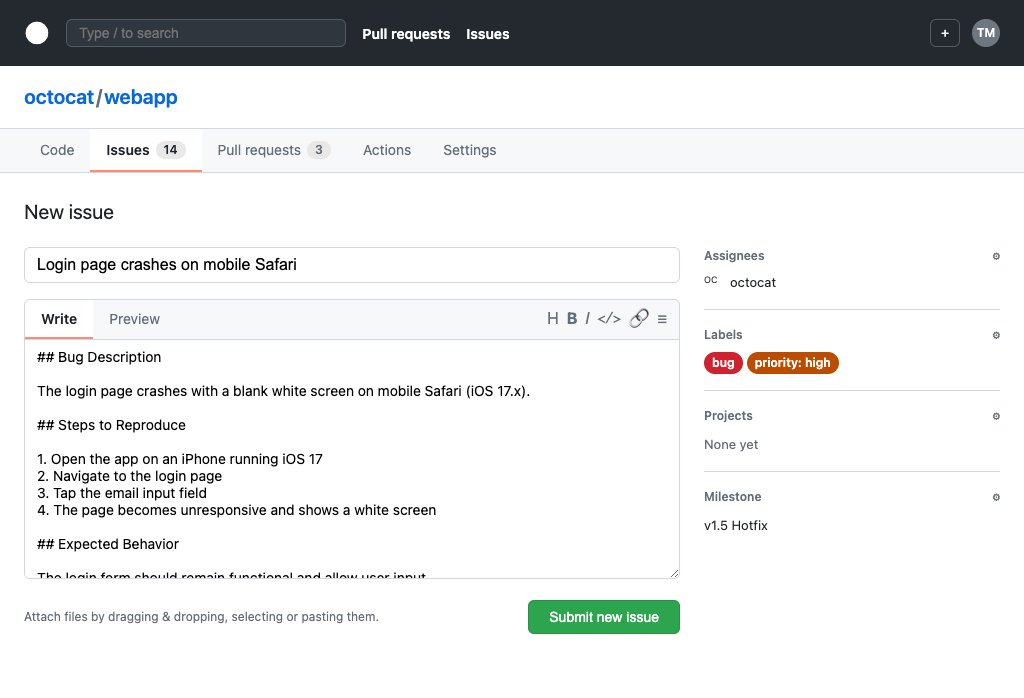
\includegraphics[width=0.95\textwidth]{images/issue-create.png}
\caption{Issue作成画面。タイトル入力欄、本文のMarkdownエディタ、右サイドバーのラベル・担当者設定が見える状態}
\end{figure}

本文ではMarkdownが使えるため、見出し、箇条書き、コードブロック、画像の貼り付けなど、リッチな記述が可能です。また、画像はドラッグ\&ドロップで簡単に添付できます。

\subsection{GitHub CLI（gh）での作成}

ターミナルで作業している場合、ブラウザに切り替えることなくIssueを作成できるのがGitHub CLIの利点です。

\begin{lstlisting}[language=bash]
# 対話形式で作成（タイトルや本文を順に聞かれる）
gh issue create

# タイトルと本文を直接指定
gh issue create --title "ログイン画面が表示されない" --body "トップページからログインボタンを押すと画面が白くなる"

# ラベルと担当者も同時に指定
gh issue create --title "ダークモード対応" --label "enhancement" --assignee "@me"

# マイルストーンも指定する場合
gh issue create --title "パフォーマンス改善" --label "enhancement" --milestone "v2.0"
\end{lstlisting}

対話形式（\cmd{gh issue create} を引数なしで実行）では、エディタが開いて本文を編集できるため、長い説明を書く場合にも便利です。コマンドライン派の開発者にとっては、コードを書いている最中に思いついたバグや改善点をすぐにIssue化できるため、作業の流れを中断せずに済みます。

\section{良いIssueの書き方}

Issueは「書けば終わり」ではなく、他の人（あるいは未来の自分）が読んで理解できることが大切です。曖昧なIssueは対応の遅れや誤解の原因になります。ここでは、バグ報告と機能要望のそれぞれについて、効果的な書き方を解説します。

\subsection{バグ報告のテンプレート}

バグ報告で最も重要なのは\textbf{再現性}です。開発者がそのバグを自分の環境で再現できなければ、修正は困難です。そのため、以下の4つの要素を必ず含めるようにしましょう。

\begin{enumerate}
  \item \textbf{再現手順（Steps to Reproduce）} --- バグに至るまでの操作を、誰でもたどれるように順を追って書く
  \item \textbf{期待する動作（Expected Behavior）} --- 本来はどうなるべきだったか
  \item \textbf{実際の動作（Actual Behavior）} --- 実際に何が起きたか
  \item \textbf{環境（Environment）} --- OS、ブラウザ、アプリのバージョンなど
\end{enumerate}

具体的な例を見てみましょう。

\begin{lstlisting}[language={}]
## バグの概要
ログインページで「パスワードを忘れた」リンクが機能しない

## 再現手順
1. https://example.com/login にアクセスする
2. 「パスワードを忘れた方はこちら」リンクをクリックする
3. 404エラーが表示される

## 期待する動作
パスワードリセットページが表示され、メールアドレスの入力フォームが現れる

## 実際の動作
404 Not Found エラーページが表示される

## 環境
- OS: macOS 14.2
- ブラウザ: Chrome 120.0.6099.109
- アプリバージョン: v2.3.1

## スクリーンショット
（ここにエラー画面のスクリーンショットを貼付）
\end{lstlisting}

ポイントは、「パスワードリセットが壊れている」のような曖昧な報告ではなく、具体的な操作手順と、期待と実際の差分を明示することです。スクリーンショットやエラーログがあれば、さらに診断が容易になります。

\subsection{機能要望の書き方}

機能要望では、「何がほしいか」だけでなく「なぜほしいか」を伝えることが重要です。開発チームは限られたリソースの中で優先順位を判断する必要があるため、背景や理由が明確であるほど、提案が採用されやすくなります。

\begin{lstlisting}[language={}]
## 概要
ダークモードに対応してほしい

## 背景・理由
- 夜間に長時間作業するユーザーが多く、目の疲れが報告されている
- 競合製品（ProductX, ProductY）はすでに対応済み
- アクセシビリティの観点からも、表示モードの選択肢があることが望ましい

## 提案する実装
- システムのダーク/ライト設定に連動する自動切り替え
- ユーザー設定画面での手動切り替えオプション
- 各UIコンポーネントでのカラーテーマ対応

## 参考情報
- デザインガイドライン案: https://example.com/dark-mode-guide
- 関連Issue: #28（カラーテーマの要望）
\end{lstlisting}

\section{ラベル（Labels）}

\subsection{ラベルの役割}

ラベルは、Issueに付ける\textbf{色付きのタグ}です。ラベルを付けることで、大量のIssueの中から特定の種類のものをすばやく絞り込むことができます。たとえば、「バグだけを見たい」「フロントエンド関連の未対応タスクだけを一覧したい」といった場面で威力を発揮します。

本のしおりやファイルのインデックスタブを想像してください。ラベルはまさにそのデジタル版であり、Issueを多角的に分類するための仕組みです。1つのIssueに複数のラベルを付けることもできるため、「バグ」かつ「フロントエンド」かつ「高優先度」のように、複数の軸で分類が可能です。

\subsection{デフォルトラベル一覧}

GitHubでリポジトリを新規作成すると、以下のラベルが自動的に用意されます。

\begin{tabular}{|l|l|l|}
\hline
\textbf{ラベル名} & \textbf{色} & \textbf{意味・用途} \\
\hline
\cmd{bug} & 赤 & ソフトウェアのバグ報告 \\
\hline
\cmd{enhancement} & 水色 & 既存機能の改善や新機能の追加提案 \\
\hline
\cmd{documentation} & 紫 & ドキュメントの追加・修正 \\
\hline
\cmd{good first issue} & 緑 & 初心者が取り組みやすい課題 \\
\hline
\cmd{help wanted} & 黄 & 外部からの助けを求めている課題 \\
\hline
\cmd{question} & ピンク & 質問や不明点の相談 \\
\hline
\cmd{duplicate} & グレー & 既存のIssueと重複している \\
\hline
\cmd{invalid} & グレー & 有効でない（再現できない、仕様どおりなど） \\
\hline
\cmd{wontfix} & 白 & 対応しないと判断された課題 \\
\hline
\end{tabular}

\subsection{カスタムラベルの作成}

デフォルトラベルだけでは足りない場合、プロジェクトの特性に合わせたカスタムラベルを作成できます。Web UIでは Issues タブ → Labels → 「New label」から作成できます。CLIでは以下のように操作します。

\begin{lstlisting}[language=bash]
# 優先度ラベル
gh label create "priority:high" --color "FF0000" --description "高優先度 — 即座に対応が必要"
gh label create "priority:medium" --color "FFA500" --description "中優先度"
gh label create "priority:low" --color "0E8A16" --description "低優先度"

# 領域ラベル
gh label create "frontend" --color "1D76DB" --description "フロントエンド関連"
gh label create "backend" --color "E4E669" --description "バックエンド関連"
gh label create "infrastructure" --color "D4C5F9" --description "インフラ・DevOps関連"
\end{lstlisting}

\begin{figure}[htbp]
\centering
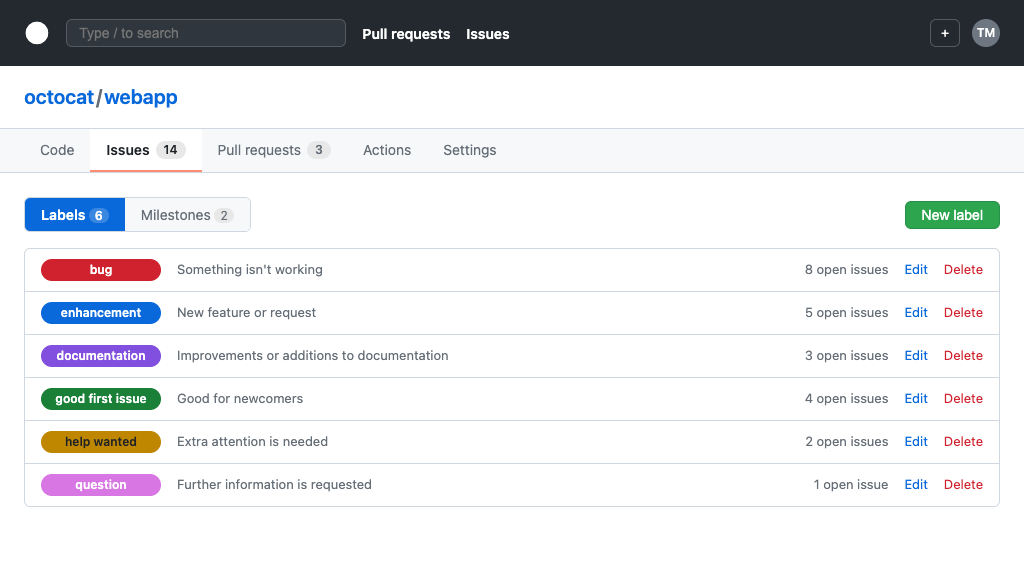
\includegraphics[width=0.95\textwidth]{images/issue-labels.png}
\caption{ラベル管理画面。色付きのラベルが一覧表示されている状態}
\end{figure}

ラベルの命名規則として、\cmd{priority:high} や \cmd{area:frontend} のように\textbf{カテゴリ:値}の形式を使うと、多数のラベルがあっても整理しやすくなります。色も、同じカテゴリのラベルには同系色を使うと視覚的にグルーピングできて便利です。

\section{マイルストーン（Milestones）}

\subsection{マイルストーンとは}

マイルストーンは、複数のIssueを\textbf{リリースや期限といった大きなゴールでグループ化}する機能です。たとえば「v2.0リリース」というマイルストーンを作り、そのリリースに必要なIssueを紐づけておくと、進捗がパーセンテージで表示され、リリースに向けてあとどれくらいの作業が残っているかが一目で分かります。

登山の「マイルストーン（里程標）」と同じ発想です。頂上（リリース）に至るまでの中間地点を設定しておくことで、今どこまで進んでいるのかを把握できるようになります。

\subsection{マイルストーンの作成と管理}

Web UIでは、Issues タブ → Milestones → 「New milestone」から作成します。CLIからはGitHub APIを直接呼び出します。

\begin{lstlisting}[language=bash]
# マイルストーンの作成
gh api repos/{owner}/{repo}/milestones \
  -f title="v2.0" \
  -f description="バージョン2.0リリース — ダークモードと多言語対応を含む" \
  -f due_on="2026-06-30T00:00:00Z"
\end{lstlisting}

マイルストーンには以下の情報を設定できます。

\begin{itemize}
  \item \textbf{タイトル} --- \cmd{v2.0}、\cmd{Sprint 3}、\cmd{2026年Q2} など
  \item \textbf{期限（Due date）} --- オプションですが、設定すると期限超過の際に警告が表示されます
  \item \textbf{説明} --- このマイルストーンのゴールや含まれる主要な変更を記述します
\end{itemize}

Issueをマイルストーンに紐づけるには、Issueの右サイドバーから設定するか、CLIでIssue作成時に \cmd{--milestone "v2.0"} を指定します。マイルストーン内のIssueがすべてクローズされると、進捗バーが100\%になり、マイルストーン自体をクローズできます。

\begin{figure}[htbp]
\centering
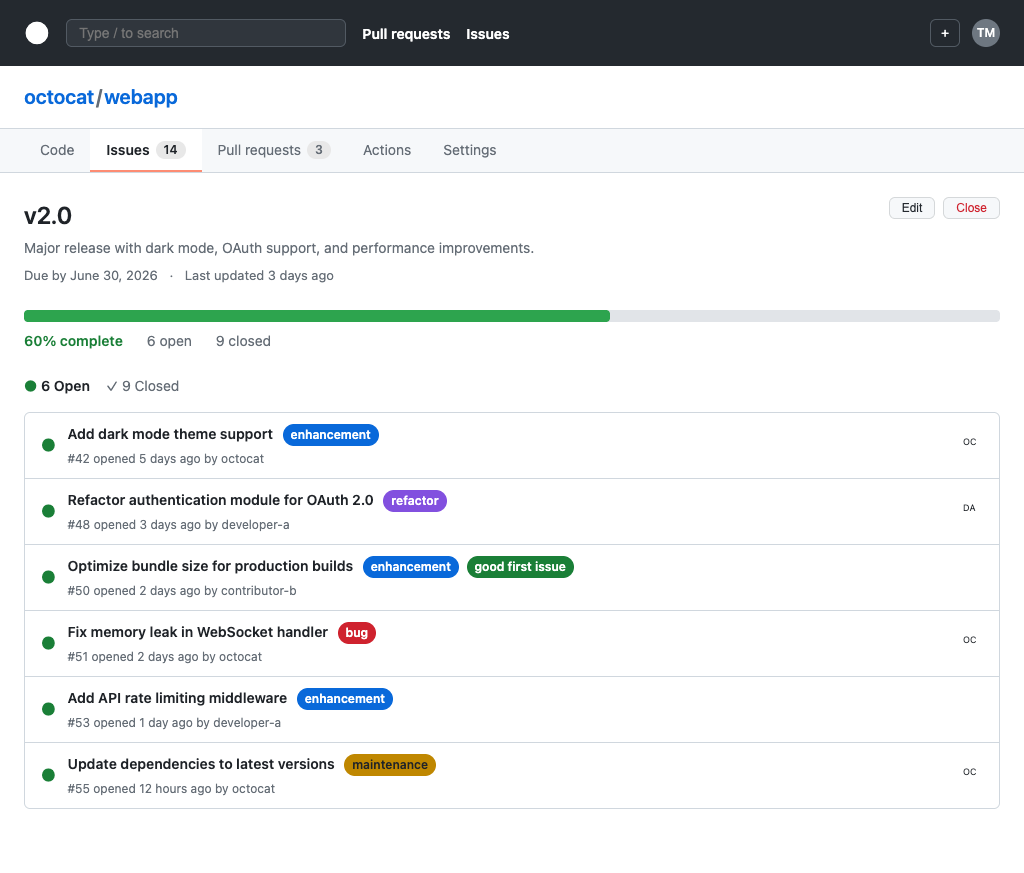
\includegraphics[width=0.95\textwidth]{images/issue-milestone.png}
\caption{マイルストーンの進捗画面。進捗バーとOpen/Closedの件数が表示されている状態}
\end{figure}

\section{IssueとPull Requestの連携}

\subsection{自動クローズキーワード}

GitHubの非常に便利な機能の1つが、\textbf{Pull RequestのマージによるIssueの自動クローズ}です。PRの本文（Description）やコミットメッセージに特定のキーワードとIssue番号を書いておくと、そのPRがデフォルトブランチにマージされた時点で、該当のIssueが自動的にクローズされます。

使えるキーワードは以下のとおりです（大文字・小文字は区別されません）。

\begin{tabular}{|l|l|}
\hline
\textbf{キーワード} & \textbf{例} \\
\hline
\cmd{Closes} & \cmd{Closes \#42} \\
\hline
\cmd{Fixes} & \cmd{Fixes \#42} \\
\hline
\cmd{Resolves} & \cmd{Resolves \#42} \\
\hline
\end{tabular}

これらはすべて同じ動作をしますが、ニュアンスの違いで使い分けると読みやすくなります。バグ修正なら \cmd{Fixes \#42}、機能実装なら \cmd{Closes \#42}、議論の解決なら \cmd{Resolves \#42} といった具合です。

複数のIssueを同時にクローズすることもできます。

\begin{lstlisting}[language={}]
## このPRで対応した内容

- ログイン画面の404エラーを修正 (Fixes #42)
- パスワードリセット機能のUIを改善 (Closes #43)
- 関連するテストを追加 (Closes #44)
\end{lstlisting}

この連携の重要なポイントは、「なぜこのコード変更が行われたか」が自動的に追跡可能になることです。Issue \cmd{\#42} を見れば修正PRへのリンクがあり、PRを見ればどのIssueに対応したかが分かる。この双方向のトレーサビリティが、プロジェクト管理の質を大きく向上させます。

\subsection{コミットメッセージでの参照}

PR本文だけでなく、コミットメッセージにもIssue番号を含めることが推奨されます。

\begin{lstlisting}[language=bash]
git commit -m "Fix password reset link returning 404 (#42)"
\end{lstlisting}

\cmd{\#42} と書くだけで（キーワードなしでも）GitHub上で自動的にリンクが生成され、該当Issueのタイムラインにも参照が表示されます。ただし、自動クローズされるのはキーワード付きの場合のみです。

\section{Issueテンプレート}

\subsection{テンプレートの必要性}

チームでの開発では、Issueの品質にばらつきが出がちです。ある人は詳細なバグ報告を書いてくれますが、別の人は「動かない」としか書いてくれないかもしれません。Issueテンプレートを用意しておくと、「New issue」をクリックした時点であらかじめ必要な項目が表示されるため、記入漏れを防ぐことができます。

テンプレートは \cmd{.github/ISSUE\_TEMPLATE/} ディレクトリにYAMLファイルとして配置します。複数のテンプレートを用意すると、Issue作成時に「バグ報告」「機能要望」などから選択する画面が表示されます。

\begin{figure}[htbp]
\centering
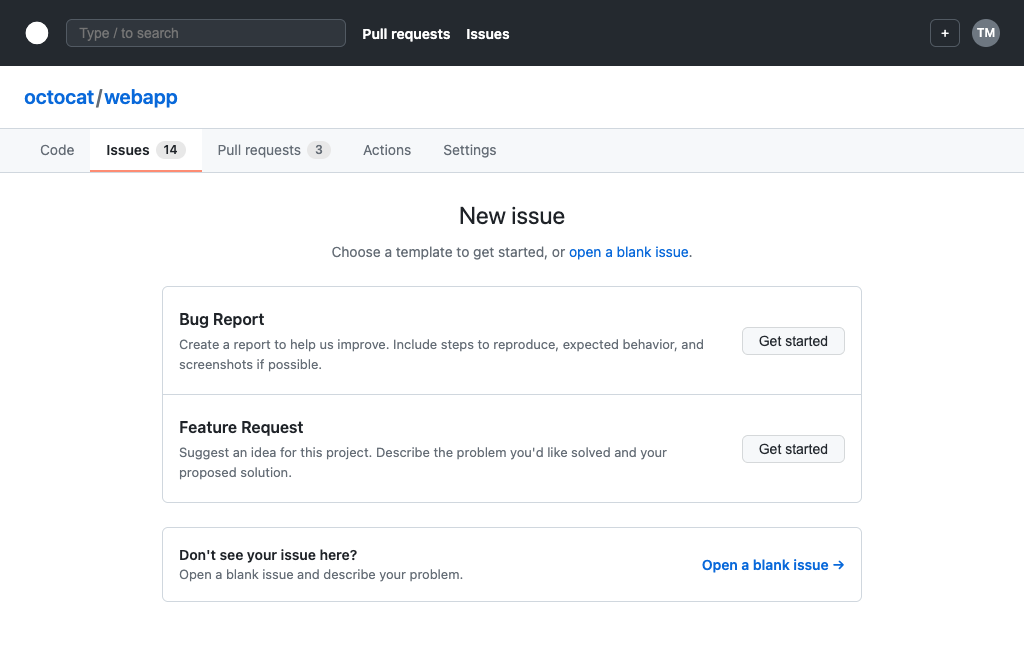
\includegraphics[width=0.95\textwidth]{images/issue-template-select.png}
\caption{Issueテンプレート選択画面。「バグ報告」「機能要望」の選択肢が表示されている状態}
\end{figure}

\subsection{バグ報告テンプレートの作成}

以下は、YAML形式のバグ報告テンプレートの例です。GitHubのフォーム機能を使うことで、自由記述だけでなくドロップダウンやチェックボックスも利用できます。

\begin{lstlisting}[language={}]
# .github/ISSUE_TEMPLATE/bug_report.yml
name: バグ報告
description: バグを報告する
title: "[Bug]: "
labels: ["bug"]
body:
  - type: textarea
    id: description
    attributes:
      label: バグの概要
      description: 何が起きていますか？簡潔に説明してください。
    validations:
      required: true
  - type: textarea
    id: steps
    attributes:
      label: 再現手順
      description: バグを再現するための手順を記述してください。
      value: |
        1. '...' に移動する
        2. '...' をクリックする
        3. エラーが表示される
    validations:
      required: true
  - type: textarea
    id: expected
    attributes:
      label: 期待する動作
      description: 本来はどのように動作すべきですか？
    validations:
      required: true
  - type: textarea
    id: actual
    attributes:
      label: 実際の動作
      description: 実際にはどのように動作しましたか？
    validations:
      required: true
  - type: dropdown
    id: os
    attributes:
      label: OS
      options:
        - macOS
        - Windows
        - Linux
        - iOS
        - Android
    validations:
      required: true
  - type: input
    id: version
    attributes:
      label: アプリバージョン
      placeholder: "例: v2.3.1"
    validations:
      required: false
\end{lstlisting}

\subsection{機能要望テンプレートの作成}

\begin{lstlisting}[language={}]
# .github/ISSUE_TEMPLATE/feature_request.yml
name: 機能要望
description: 新機能を提案する
title: "[Feature]: "
labels: ["enhancement"]
body:
  - type: textarea
    id: problem
    attributes:
      label: 解決したい課題
      description: この機能がないことで、どのような問題がありますか？
    validations:
      required: true
  - type: textarea
    id: solution
    attributes:
      label: 提案する解決策
      description: どのような機能を実装すれば解決しますか？
    validations:
      required: true
  - type: textarea
    id: alternatives
    attributes:
      label: 検討した代替案
      description: 他に検討した方法があれば記述してください。
    validations:
      required: false
\end{lstlisting}

\cmd{validations: required: true} を設定すると、その項目が未記入のままではIssueを送信できなくなります。これにより、必要最低限の情報が常に揃ったIssueが作成されるようになります。

\section{Issueの管理}

\subsection{CLIでの操作}

日常的なIssue管理は、GitHub CLIを使うとブラウザを開かずに素早く行えます。

\begin{lstlisting}[language=bash]
# Issue一覧を表示（デフォルトではOpen状態のIssueが表示される）
gh issue list

# 特定のラベルが付いたIssueだけを表示
gh issue list --label "bug"

# 自分に割り当てられたIssueを表示
gh issue list --assignee "@me"

# クローズ済みのIssueも含めて表示
gh issue list --state all

# 特定のIssueの詳細を表示
gh issue view 42

# ブラウザで開く（詳細な確認やコメントの画像添付が必要な場合に便利）
gh issue view 42 --web

# Issueをクローズする
gh issue close 42

# Issueを再オープンする
gh issue reopen 42

# Issueにコメントを追加する
gh issue comment 42 --body "修正PRを作成しました: #45 を確認してください"

# Issueにラベルを追加する
gh issue edit 42 --add-label "priority:high"

# Issueの担当者を変更する
gh issue edit 42 --add-assignee "alice"
\end{lstlisting}

\subsection{ピン留め（Pinned Issues）}

特に重要なIssue――たとえばプロジェクトの行動規範、コントリビューションガイドライン、既知の重大バグなど――は、IssuesタブのTopに固定表示（ピン留め）することができます。最大3つまでピン留めが可能です。

ピン留めの方法は、該当Issueを開き、右サイドバーの「\textbf{Pin issue}」をクリックするだけです。ピン留めされたIssueはIssues一覧の最上部に表示されるため、リポジトリを訪れた人が最初に目にすることになります。

\begin{figure}[htbp]
\centering
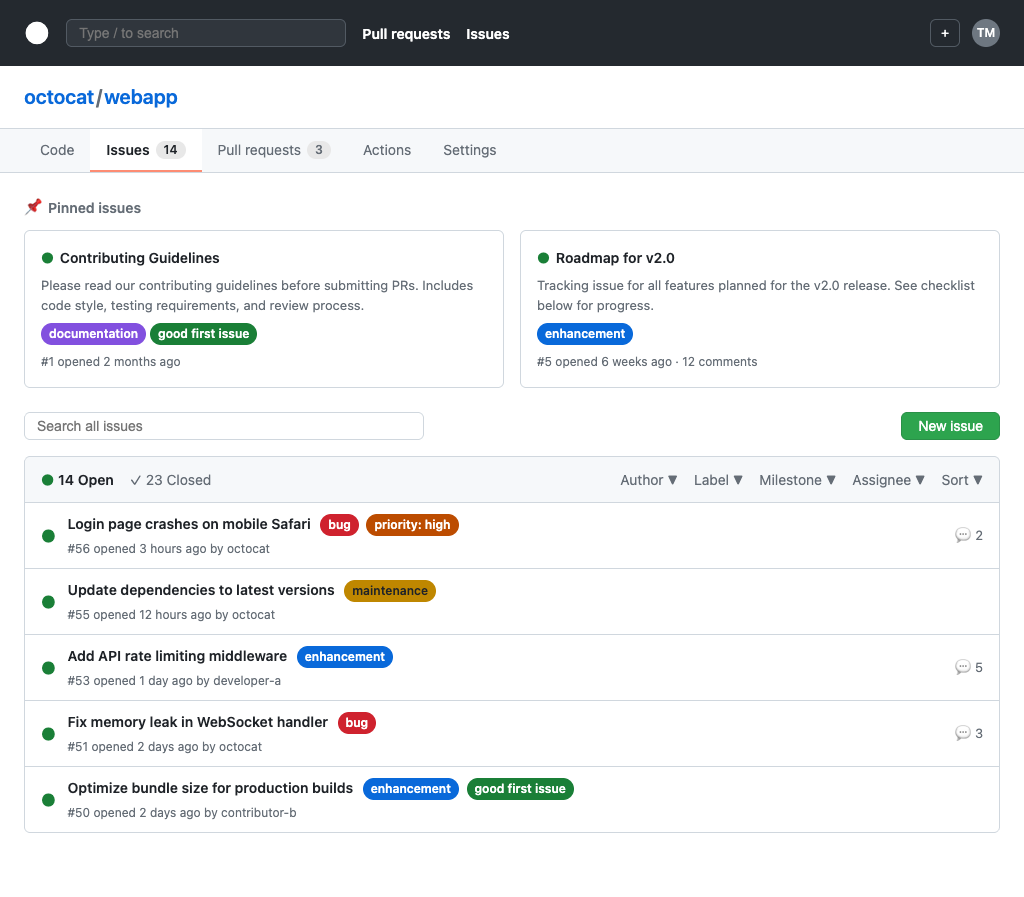
\includegraphics[width=0.95\textwidth]{images/issue-pinned.png}
\caption{ピン留めされたIssueがIssues一覧の上部に表示されている状態}
\end{figure}

\subsection{Issueの検索とフィルタリング}

Issueが増えてくると、効率的な検索が不可欠です。GitHub Webの検索バーでは、以下のようなフィルタが使えます。

\begin{tabular}{|l|l|l|}
\hline
\textbf{フィルタ} & \textbf{例} & \textbf{意味} \\
\hline
\cmd{is:open} & \cmd{is:open label:bug} & Open状態のバグ \\
\hline
\cmd{is:closed} & \cmd{is:closed milestone:v2.0} & v2.0マイルストーンのクローズ済みIssue \\
\hline
\cmd{assignee:} & \cmd{assignee:alice} & aliceに割り当てられたIssue \\
\hline
\cmd{author:} & \cmd{author:bob} & bobが作成したIssue \\
\hline
\cmd{no:label} & \cmd{no:label is:open} & ラベルが付いていない未対応Issue \\
\hline
\end{tabular}

これらのフィルタを組み合わせることで、必要なIssueをすばやく見つけることができます。

\section{まとめ}

この章では、GitHubのIssue機能を包括的に学びました。重要なポイントを振り返ります。

\begin{itemize}
  \item \textbf{Issueはチケットシステム}であり、バグ報告・機能要望・タスク管理・議論のすべてを1箇所で管理できます
  \item \textbf{Issue番号はPRと共通の通し番号}であり、コミットメッセージやPRから \cmd{\#番号} で参照できます
  \item \textbf{良いIssue}は、再現手順・期待動作・実際の動作・環境情報を含む具体的なものです
  \item \textbf{ラベル}でIssueを分類し、\textbf{マイルストーン}でリリースや期限ごとにグループ化することで、プロジェクトの全体像を把握しやすくなります
  \item \cmd{Closes \#42} などのキーワードにより、\textbf{PRのマージでIssueを自動クローズ}できます
  \item \textbf{テンプレート}を用意することで、チーム全体のIssue品質を一定に保つことができます
\end{itemize}

Issueを適切に活用することは、単にタスクを管理するだけでなく、プロジェクトの意思決定の記録を残すことでもあります。「なぜこの機能をこのように実装したのか」という判断の背景が、Issueの議論の中に残っていれば、後からプロジェクトに参加したメンバーも文脈を理解できます。
